\pagebreak
\section{Результаты}

\textbf{Сравнение времени работы}

В качестве замеров времени используем усредненное время выполнения функции \texttt{update} на первой 1000 кадров, при различном количестве сфер. Конфигурация ядра обработки сфер: необходимое количество блоков размером 256. Конфигурация ядра обработки пола фиксированная: $32\times32$, $32\times8$. Разрешение текстуры карты напряженности: $100\times100$.

\begin{center}
\begin{tabular}{|l*{6}{|r}|}
\hline
\textbf{Конфигурация} & \multicolumn{6}{c|}{\textbf{Время выполнения, мс}} \\
\hline
\hline
\textbf{Количество объектов} & 10 & 50 & 100 & 150 & 250 & 500 \\
\hline
CPU & 2.154 & 8.680 & 17.878 & 28.564 & 50.055 & 121.930  \\
\hline
GPU & 16.133 & 15.731 & 15.159 & 14.731 & 23.046 & 44.266 \\
\hline
\hline
\textbf{Количество объектов} & 750 & 1000 & 1500 & 2000 & 2500 & \\
\hline
CPU & 223.624 & 332.131 &  &  &  & \\
\hline
GPU & 65.126 & 86.098 & 128.968 & 187.829 & 234.696 & \\
\hline
\end{tabular}
\end{center}

Из-за фиксированных конфигураций, время выполнения параллельной версии практически не отличается при маленьком количестве сфер, однако при 250 и более ее преимущество перед CPU версией более чем очевидно. При 1500 объектов производительность CPU версии падает до 2 fps, поэтому ее тестирование было остановлено на этом. GPU версия при таком количестве работает с 10 fps, что позволяет увеличивать его дальше, но при 2500 объектов их становится так много, что часть выдавливается за стенки куба.

\begin{tikzpicture}
\begin{axis}[
    ylabel = Время выполнения (мс),
    xlabel = Количество объектов,
    xtick = {10, 100, 250, 500, 750, 1000, 1500, 2000, 2500},
    width = .98\textwidth,
    height = .7\textwidth,
    legend pos = south east,
    colormap name = colormap/jet,
    cycle list = {[of colormap]}
]
\legend{
    CPU,
    GPU,
};
\pgfplotstableread{data/time.dat}\timetable
\addplot+ [thick, mark=*] table [x=count, y=cpu] {\timetable};
\addplot+ [thick, mark=*] table [x=count, y=gpu] {\timetable};
\end{axis}
\end{tikzpicture}
\pagebreak

\textbf{Результаты работы}

\begin{figure}[h]
\centering
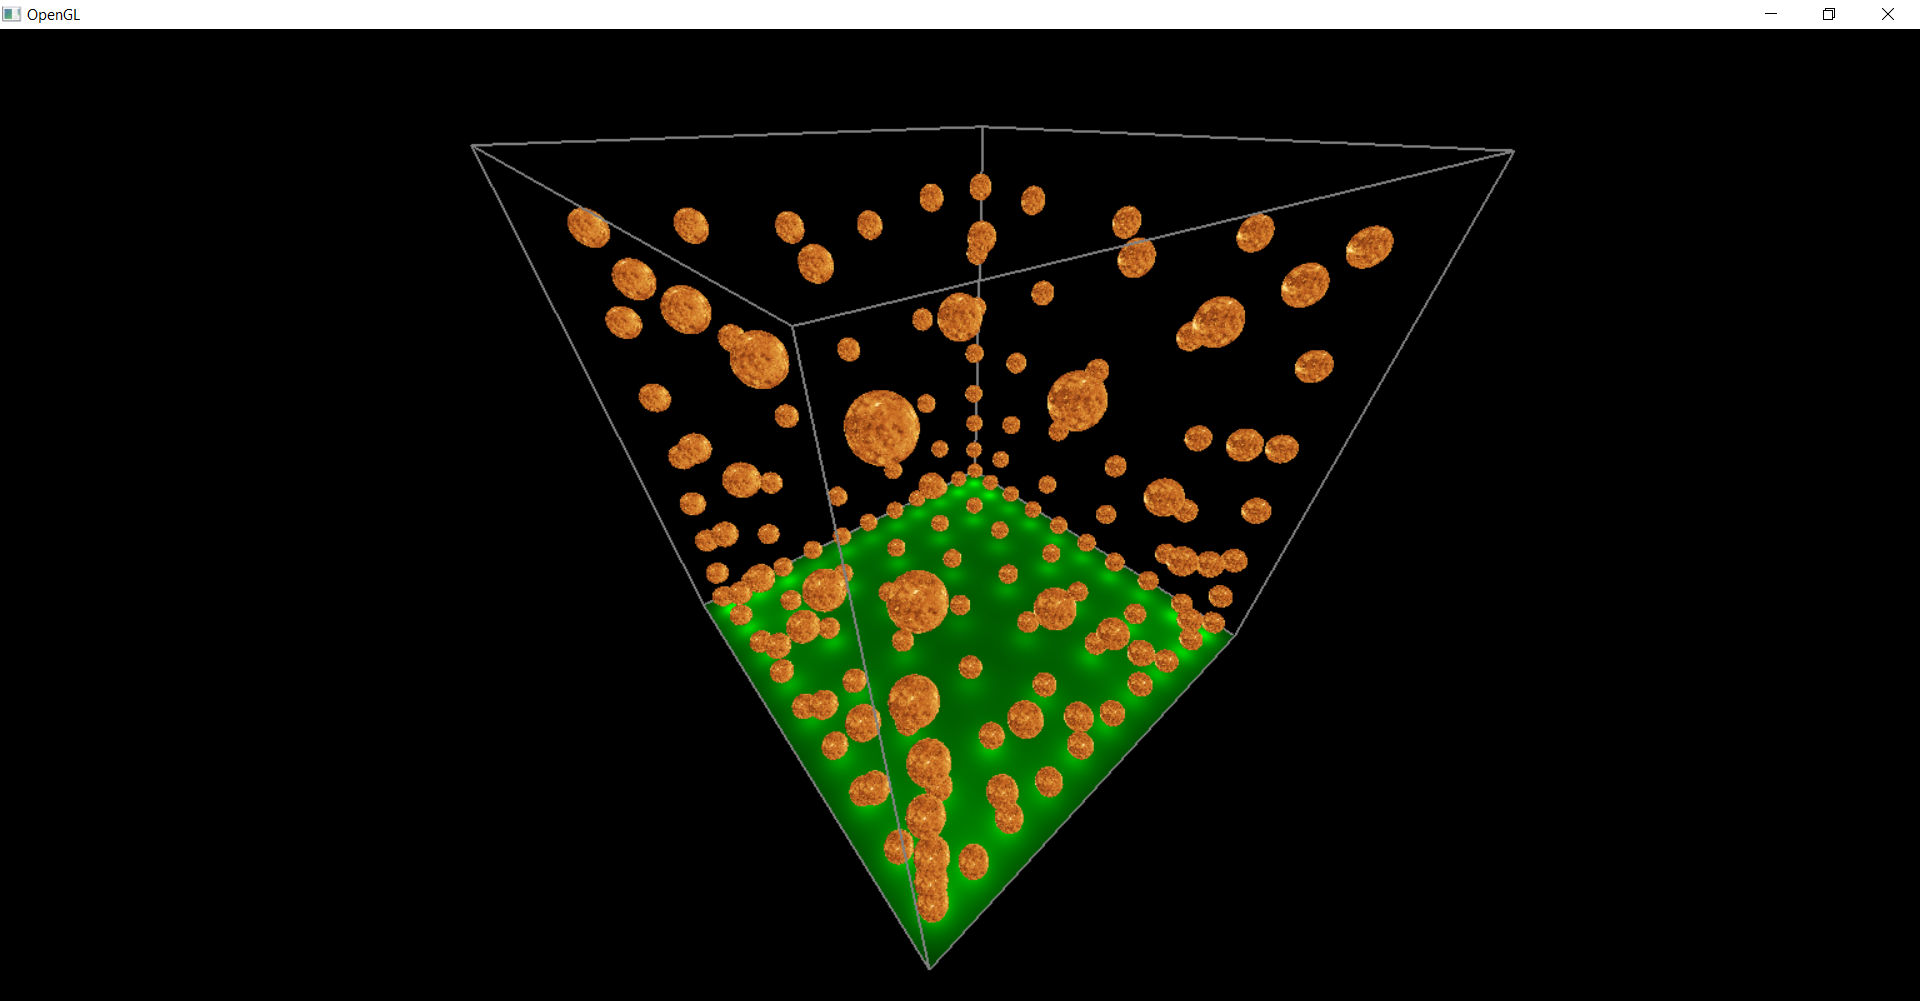
\includegraphics[width=.97\textwidth]{balance}
\caption{Состояние равновесия}
\end{figure}

\begin{figure}[h]
\centering
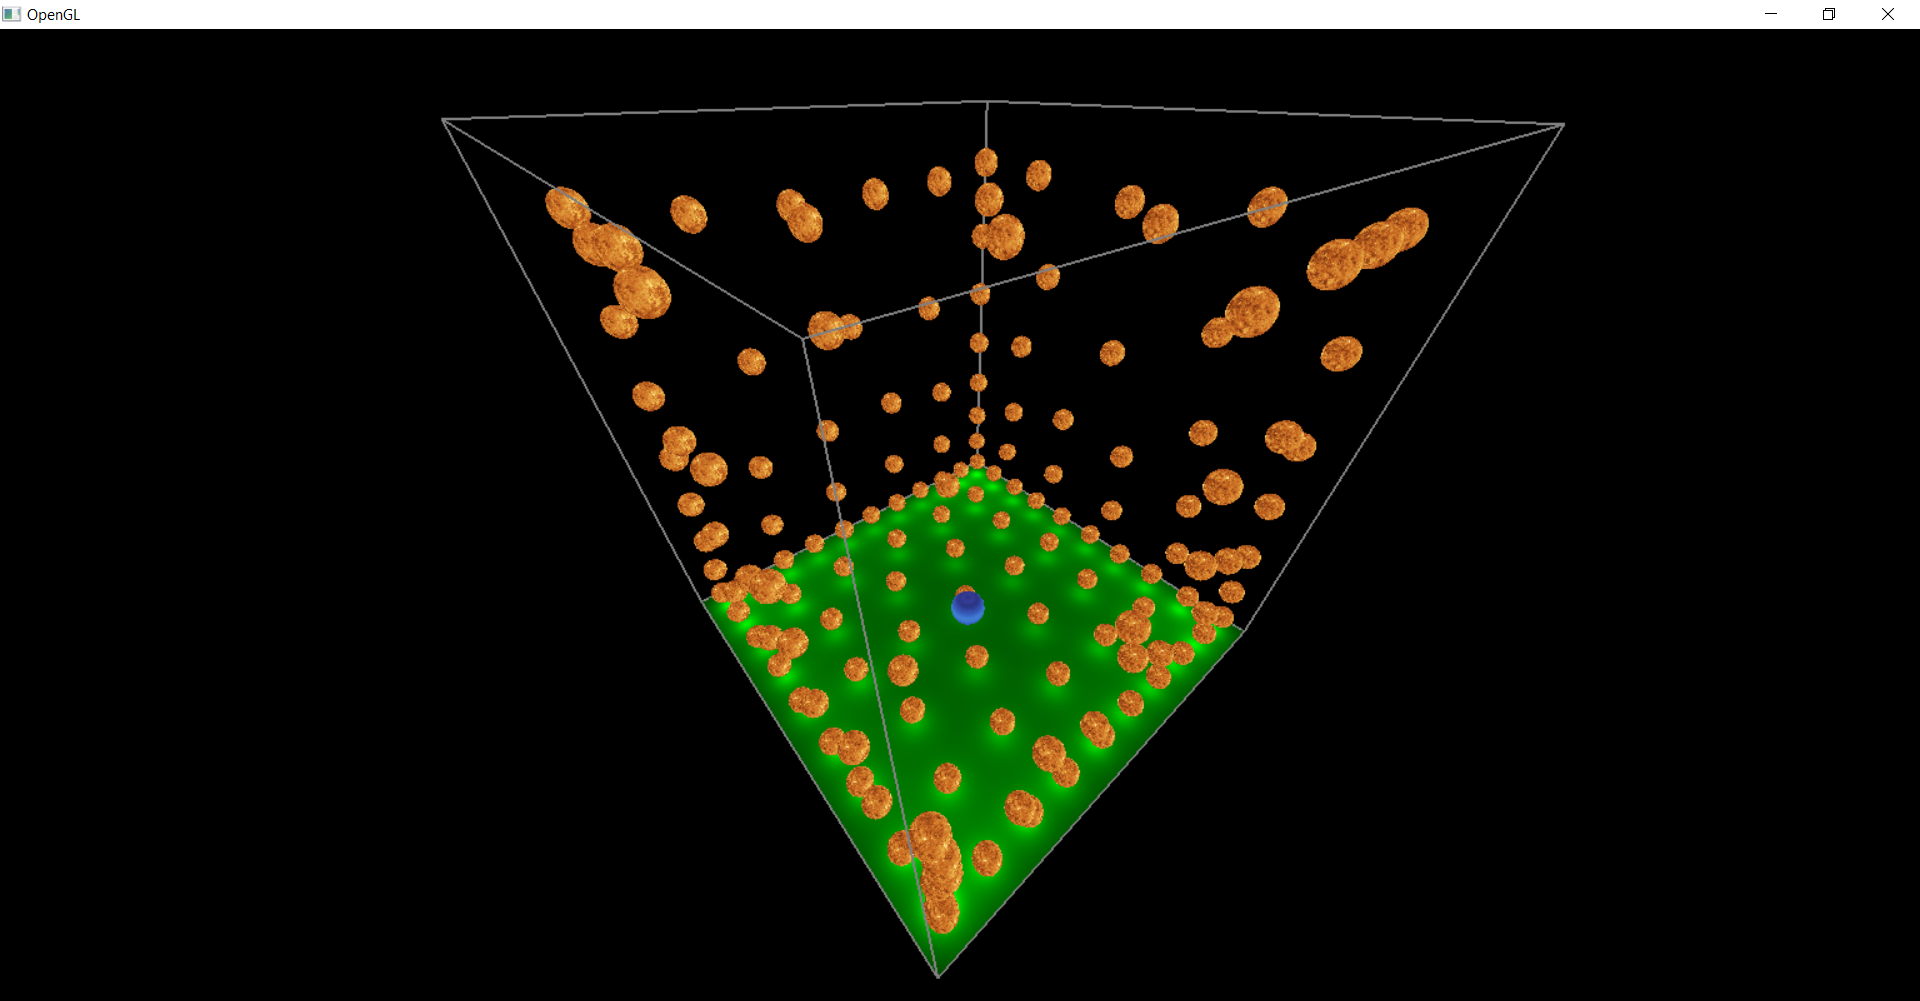
\includegraphics[width=.495\textwidth]{shot_1}\hfill
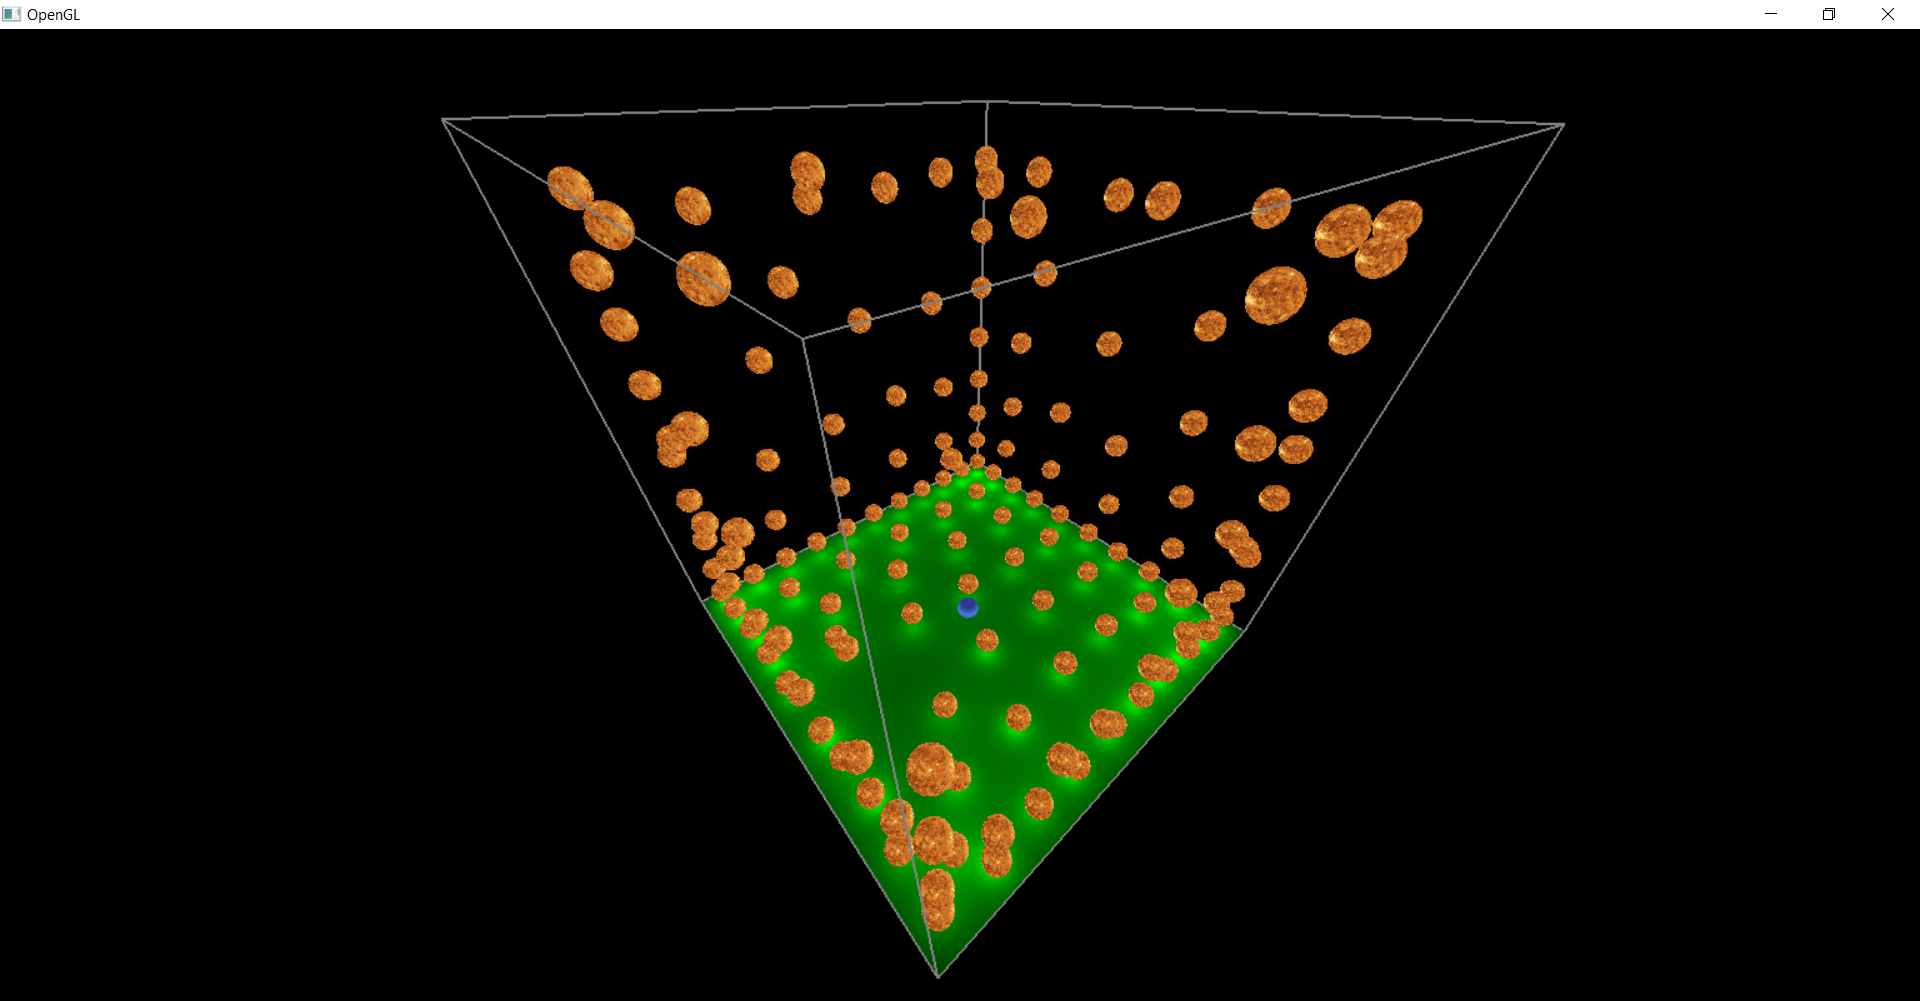
\includegraphics[width=.495\textwidth]{shot_2}
\vfill
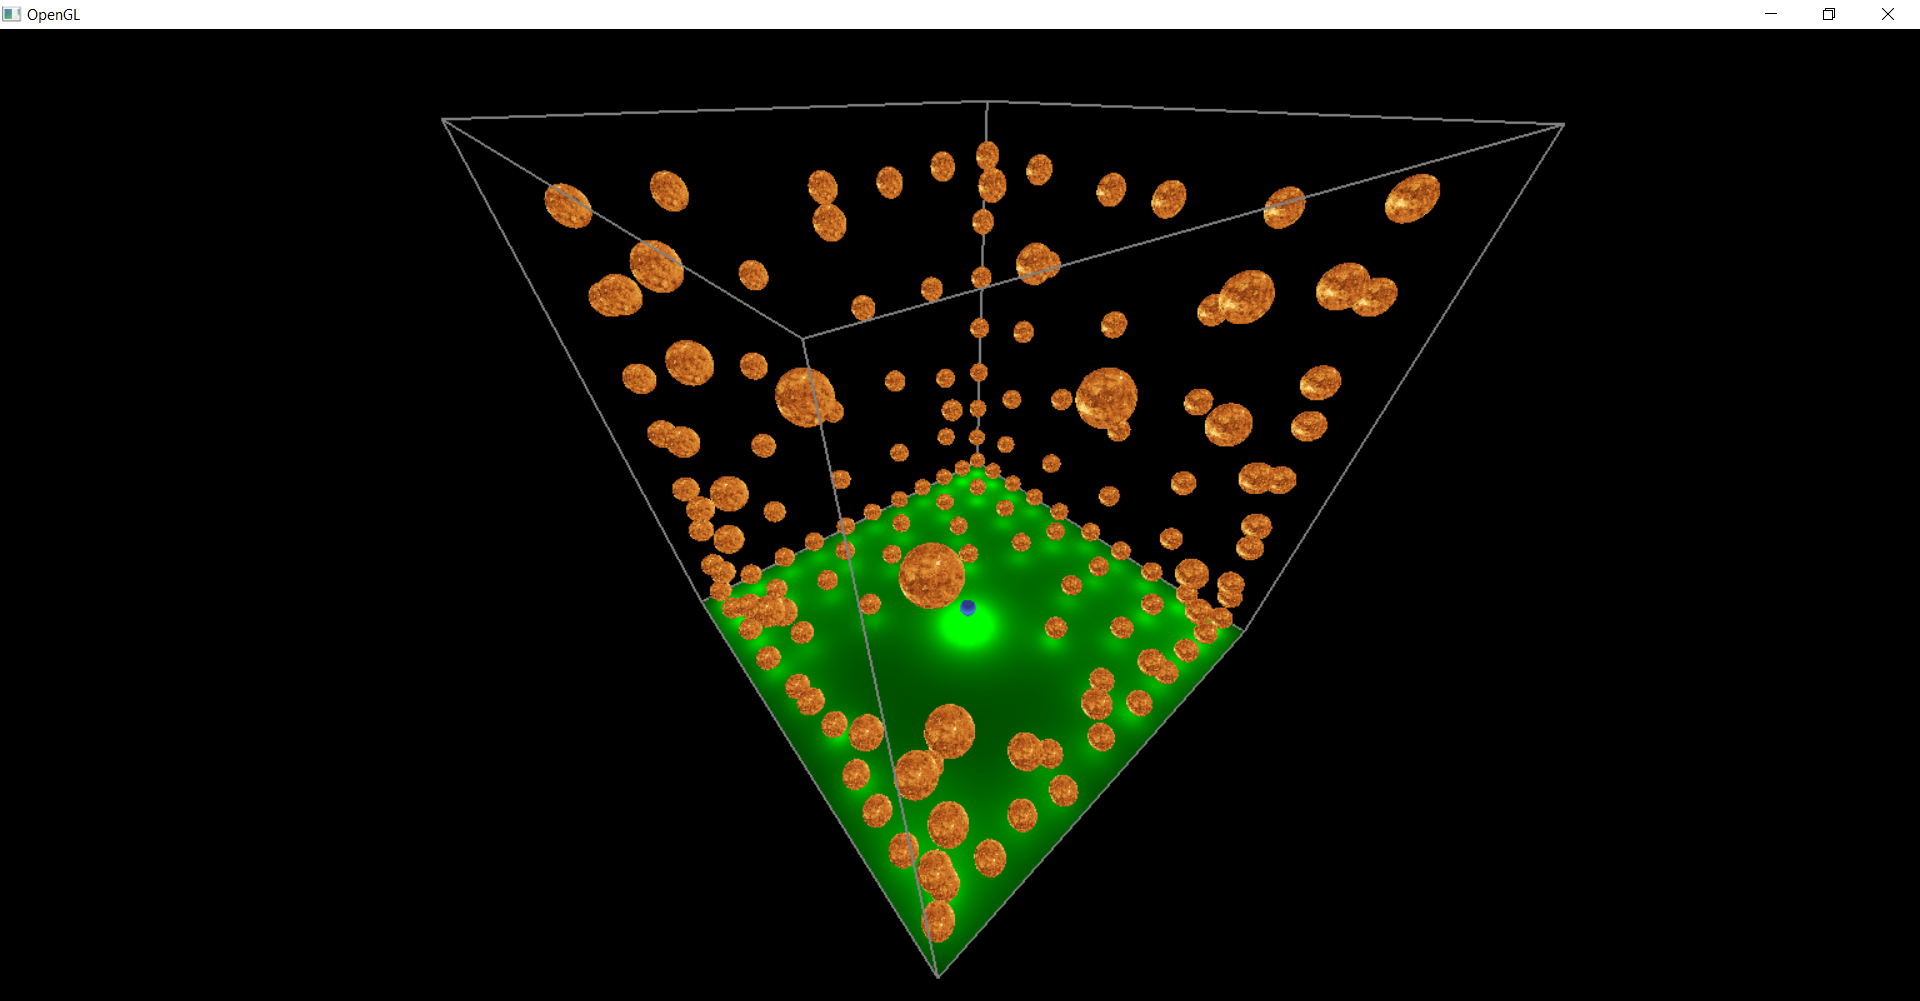
\includegraphics[width=.495\textwidth]{shot_3}
\caption{Выведение из состояния равновесия снарядом}
\end{figure}
\pagebreak
